\clearpage
\section{Hardware Primer}
\label{sec:hardware-primer}
\raggedbottom% pages end where the text ends: no stretched gaps around headings and diagrams

The Pi-Radio FR3-1ch unit is a single circuit board enclosed in a CNC-milled aluminum case; in this datasheet,
\emph{the unit} means the complete product as shipped, and \emph{the board} the circuitry inside the case. This
section is a map of that board --- what is physically on the signal path, in what
order, and how the digital side tunes and controls it --- before the rest of this datasheet gets into how each
piece actually performs. It is organized into four parts: the TX-side RF chain, the RX-side RF chain, the
clock and LO distribution shared by both of them, and the digital control layer that ties everything together.
Figure~\ref{fig:hw-photo} shows all six SMA connectors on the physical unit, labeled; the rest of this section
refers back to it by name whenever a specific connector is mentioned.

\vspace{-1em}
\begin{center}
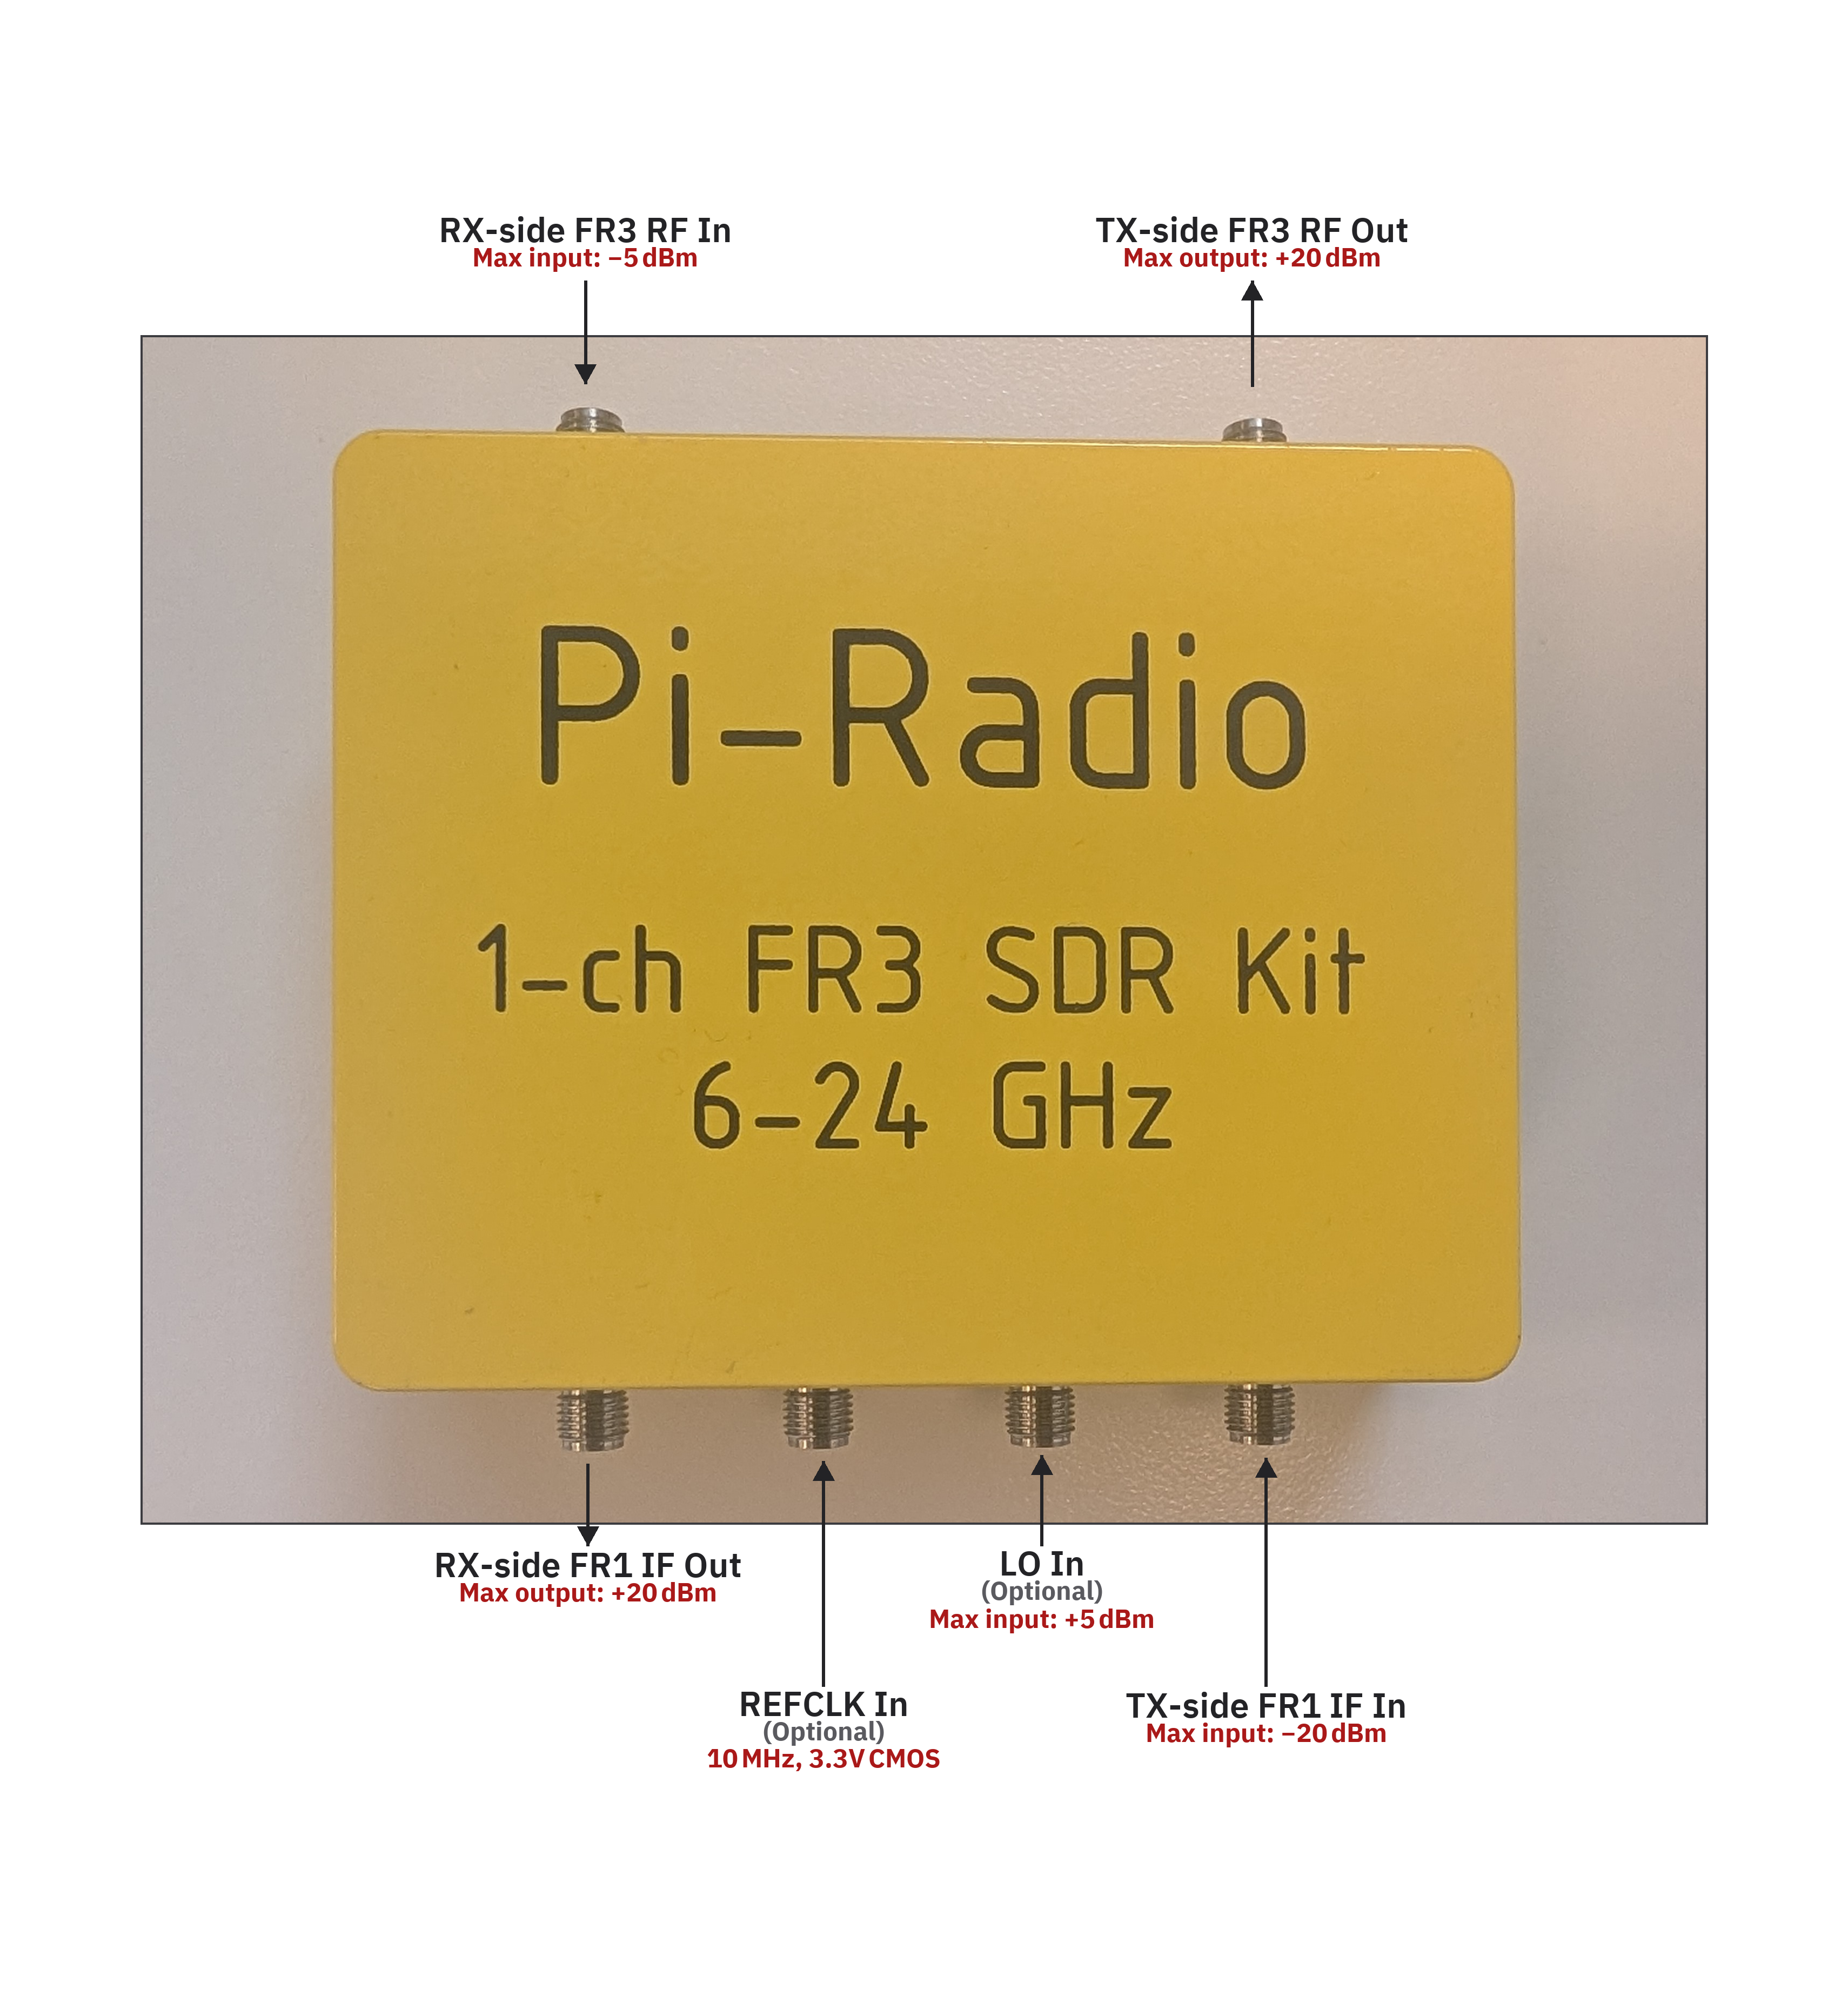
\includegraphics[width=0.56\linewidth]{images/hw_photo_labeled.png}
\vspace{-0.5em}
\captionof{figure}{The Pi-Radio FR3-1ch unit, all six SMA connectors labeled. Top row: the two FR3 (RF)
connectors. Bottom row: the two FR1 (IF) connectors and the two shared reference inputs (REFCLK, LO).}
\label{fig:hw-photo}
\end{center}
\vspace{-1.2em}

\subsection{Using the System}
\label{sec:hw-using-system}

\textbf{Why port, not rebuild.} The point of the Pi-Radio FR3-1ch unit is to let an FR1 experiment that already
works today --- a USRP, an RFSoC, a Wi-Fi chipset, a 5G modem, anything that already transmits and receives at
FR1 --- move up to FR3 without touching that system's own code at all. The existing FR1 radio keeps doing
exactly what it already does; the Pi-Radio box sits between it and the antenna and handles the up/down
conversion to and from FR3 transparently.

\textbf{TX side.} Take the transmit output of the existing FR1 system, pad it with an attenuator if its power
level calls for one, and feed it straight into the ``TX-side FR1 IF In'' connector (Figure~\ref{fig:hw-photo}).
The desired experiment --- the FR1 frequency, the target FR3 frequency, the signal bandwidth, and which sideband
to use --- is set either through the Pi-Radio GUI or directly over the USB-serial interface described in
Section~\ref{sec:hw-digital}; the unit works out the LO frequency and switch states that configuration implies
on its own. The up-converted result appears at the ``TX-side FR3 RF Out'' connector, ready to go to an antenna
or any other FR3 test setup.

\textbf{RX side.} The receive path is the mirror image of the TX path, and it is not configured separately: it
automatically takes on whatever FR1 frequency, FR3 frequency, bandwidth, and sideband the TX side was just told
to use. An FR3 signal arriving at the ``RX-side FR3 RF In'' connector comes back out as the corresponding FR1
signal at the ``RX-side FR1 IF Out'' connector, which feeds directly into the existing FR1 system's receive
input (again through an attenuator if needed).

\textbf{Phase coherence across units.} A single internal 10\,MHz TCXO and PLL/VCO (Section~\ref{sec:hw-clock-lo})
generates the one LO that both the TX and RX chains share, so a single unit's TX and RX are automatically phase
coherent with each other. Tiling several units together for multi-channel, phase-coherent operation is also
supported, with a choice of two approaches. The cheaper and simpler option distributes one common external
10\,MHz reference to every unit's ``REFCLK In'' connector through a clock buffer --- each unit still runs its
own LO, merely locked to a shared timebase. The other option distributes a single LO directly to every unit's
``LO In'' connector instead, generated by the Pi-Radio OctoLO (a phase-coherent 8-channel LO source built for
exactly this purpose), bypassing each unit's own synthesizer; this gives substantially lower phase noise
(Section~\ref{sec:phase-noise}), at the cost of needing the OctoLO itself. As a general rule of thumb, sharing one
LO keeps the units' phases more tightly aligned than sharing only the 10\,MHz reference, since each unit's own
synthesizer then no longer adds its own independent phase wander.

\textbf{Power and control.} The whole unit is powered from a single USB-C connector; the supply behind it must
be able to source 1.5\,A, since the unit draws 7.5\,W from 5\,V. If a computer's or laptop's own USB-C port
cannot source that much current directly, a powered USB-C hub in between works just as well. That same USB-C
connector also carries the
serial link used to configure everything described above --- the Pi-Radio GUI talks over this same serial
interface rather than some separate side channel, so anything the GUI can do is also reachable directly by a
script talking the same ASCII command set (Section~\ref{sec:hw-digital}).

\subsection{TX-side Up-conversion: FR1 $\to$ FR3}
\label{sec:hw-tx}

\textbf{Signal path.} An external FR1 signal (0.7--4.0\,GHz, up to 500\,MHz of instantaneous bandwidth) enters the unit's
``TX-side FR1 IF In'' connector (Figure~\ref{fig:hw-photo}) and passes through a fixed-gain amplifier (Analog
Devices ADL5545), then a 90$^\circ$ hybrid
coupler (Mini-Circuits QCH-392+) that splits it into two copies 90$^\circ$ apart in phase, FR1\_I and FR1\_Q.
These two lines pass through a DPDT switch (thru/swap) and then into the I and Q ports of a quadrature mixer
(MACOM MAMX-011075) together with the shared LO (Section~\ref{sec:hw-clock-lo}). A DC bias (I\_V, Q\_V),
produced by an on-board multi-channel DAC, is injected onto the same I/Q lines between the switch and the mixer specifically
to null the mixer's own LO-to-RF leakage (see Section~\ref{sec:lo-suppression}). After the mixer, the RF output
passes through a Mercury Systems AM3153 programmable bandpass filter, a fixed-gain LNA (HMC963), a fixed-gain final power amplifier
(Analog Devices ADL9006), and out through the ``TX-side FR3 RF Out'' connector. ``Fixed-gain'' means none of these
amplifier stages are software-adjustable --- the only thing under digital control on this path is the DPDT
switch state, the I/Q DC biases, and the AM3153 filter's selected sub-state.

\textbf{Upper vs.\ lower sideband.} The mixer is a full I/Q (quadrature) upconverter: with the DPDT switch in
``thru,'' the upper sideband dominates the RF output; in ``swap,'' the lower sideband dominates instead. This is
not merely a filter choice --- it changes which of the two possible LO frequencies the unit must tune to for a
given desired FR3 output, and whether the FR1 input's own internal spectral content comes out the same way
round or mirrored:
{\setlength{\topsep}{0.2em}\setlength{\partopsep}{0pt}\begin{itemize}\setlength{\itemsep}{0.3em}\setlength{\parskip}{0pt}
\item \textbf{Upper sideband (thru):} LO = FR3 $-$ FR1. The LO sits below FR3 (low-side). No spectral flip --- a
feature that sits at the \emph{high} end of the FR1 passband shows up at the \emph{high} end of FR3's occupied
band too.
\item \textbf{Lower sideband (swap):} LO = FR3 $+$ FR1. The LO sits above FR3 (high-side). The spectrum flips
--- a feature at the \emph{high} end of FR1 shows up at the \emph{low} end of FR3's occupied band, and vice
versa.
\end{itemize}}
Figure~\ref{fig:hw-tx-block} shows the full chain. Figure~\ref{fig:hw-tx-spectrum} shows the flip itself: the
input spectrum shown is deliberately asymmetric (steep on one edge, shallow on the other) so the mirroring is
visible at a glance in the lower-sideband case.

\noindent\begin{minipage}{\linewidth}
\centering
\begin{tikzpicture}[
  block/.style={draw, rectangle, minimum height=0.9cm, minimum width=1.7cm, align=center, font=\scriptsize,
                fill=gray!8, inner sep=3pt},
  mixblock/.style={block, fill=blue!10},
  conn/.style={draw, circle, minimum size=2pt, fill=black, inner sep=1.2pt},
  arr/.style={-{Stealth[length=2mm]}, thick},
  sidelabel/.style={font=\scriptsize, align=center},
  node distance=4.4mm  % 4.4 (not 5) so the outward connector labels keep the figure within the text width
]
\node[conn] (fr1in) {};
\node[sidelabel, anchor=south east, align=right] at ([yshift=1mm]fr1in.north east) {TX-side\\FR1 IF In};
\node[block, right=of fr1in] (amp1) {ADL5545};
\node[block, right=of amp1] (hyb) {90$^\circ$ Hybrid\\(QCH-392+)};
\node[block, right=of hyb] (dpdt) {DPDT\\thru/swap};
\node[mixblock, right=9mm of dpdt] (mix) {MAMX-011075\\Mixer};
\node[block, right=of mix] (filt) {AM3153\\Filter};
\node[block, right=of filt] (lna) {HMC963\\LNA};
\node[block, right=of lna] (pa) {ADL9006\\PA};
\node[conn, right=of pa] (fr3out) {};
\node[sidelabel, anchor=south west, align=left] at ([yshift=1mm]fr3out.north west) {TX-side\\FR3 RF Out};

\draw[arr] (fr1in) -- (amp1);
\draw[arr] (amp1) -- (hyb);
\draw[arr] ([yshift=2mm]hyb.east) -- ([yshift=2mm]dpdt.west);
\draw[arr] ([yshift=-2mm]hyb.east) -- ([yshift=-2mm]dpdt.west);
\draw[arr] ([yshift=2mm]dpdt.east) -- ([yshift=2mm]mix.west) coordinate[pos=0.5] (iline-mid);
\draw[arr] ([yshift=-2mm]dpdt.east) -- ([yshift=-2mm]mix.west) coordinate[pos=0.5] (qline-mid);
\draw[arr] (mix) -- (filt);
\draw[arr] (filt) -- (lna);
\draw[arr] (lna) -- (pa);
\draw[arr] (pa) -- (fr3out);

% LO and Q_V labels share one text baseline (anchor=base), so they sit exactly level; each arrow runs straight
% up from its label's top edge and its tip stops exactly on the target (the mixer's bottom edge / the Q line).
\coordinate (botbase) at ([yshift=-11mm]mix.south);
\node[sidelabel, anchor=base] (lo) at (mix |- botbase) {LO\\(shared)};
\draw[arr] (lo.north) -- (mix.south);
\node[sidelabel, above=7mm of iline-mid] (ibias) {I\_V\\(LO-null)};
\draw[arr] (ibias.south) -- (iline-mid);
\node[sidelabel, anchor=base] (qbias) at (qline-mid |- botbase) {Q\_V\\(LO-null)};
\draw[arr] (qbias.north) -- (qline-mid);
\end{tikzpicture}
\captionof{figure}{TX-side signal chain. Fixed-gain amplifiers and filters (grey) surround the quadrature
mixer (blue); the DPDT switch and the shared LO (Section~\ref{sec:hw-clock-lo}) together set which sideband and
which actual RF frequency come out.}
\label{fig:hw-tx-block}
\end{minipage}

\noindent\begin{minipage}{\linewidth}
\centering
\begin{tikzpicture}[font=\scriptsize]
  % ---- Panel A: Upper sideband (thru), no flip ----
  \begin{scope}[xshift=0cm]
    \node[align=center] at (0,3.1) {\textbf{Upper sideband (thru)}\\LO = FR3 $-$ FR1 (no flip)};
    \draw[-{Stealth[length=1.5mm]}] (-2.2,2) -- (2.2,2);
    \fill[blue!40] (-0.5,2) -- (-0.5,2.6) -- (0.5,2.3) -- (0.5,2) -- cycle;
    \node at (0,1.65) {FR1 (input)};
    \draw[-{Stealth[length=1.5mm]}] (-2.2,0) -- (2.2,0);
    \draw[dashed] (0,-0.15) -- (0,0.9);
    \node at (0,1.1) {LO};
    \fill[green!60] (0.9,0) -- (0.9,0.6) -- (1.9,0.3) -- (1.9,0) -- cycle;
    \node at (1.4,-0.4) {FR3 (Output)};
    \fill[red!55] (-1.9,0) -- (-1.9,0.3) -- (-0.9,0.6) -- (-0.9,0) -- cycle;
    \node at (-1.4,-0.4) {Filtered Out};
    \draw[blue!60!black, dashed, thick] (-2.2,0.05) -- (-0.9,0.05) -- (0.9,0.85) -- (2.2,0.85);
    \node[blue!60!black] at (1.4,1.05) {filter response};
  \end{scope}
  % ---- Panel B: Lower sideband (swap), flip ----
  \begin{scope}[xshift=6.4cm]
    \node[align=center] at (0,3.1) {\textbf{Lower sideband (swap)}\\LO = FR3 $+$ FR1 (flip)};
    \draw[-{Stealth[length=1.5mm]}] (-2.2,2) -- (2.2,2);
    \fill[blue!40] (-0.5,2) -- (-0.5,2.6) -- (0.5,2.3) -- (0.5,2) -- cycle;
    \node at (0,1.65) {FR1 (input)};
    \draw[-{Stealth[length=1.5mm]}] (-2.2,0) -- (2.2,0);
    \draw[dashed] (0,-0.15) -- (0,0.9);
    \node at (0,1.1) {LO};
    \fill[green!60] (-1.9,0) -- (-1.9,0.3) -- (-0.9,0.6) -- (-0.9,0) -- cycle;
    \node at (-1.4,-0.4) {FR3 (Output)};
    \fill[red!55] (0.9,0) -- (0.9,0.6) -- (1.9,0.3) -- (1.9,0) -- cycle;
    \node at (1.4,-0.4) {Filtered Out};
    \draw[blue!60!black, dashed, thick] (-2.2,0.85) -- (-0.9,0.85) -- (0.9,0.05) -- (2.2,0.05);
    \node[blue!60!black] at (-1.4,1.05) {filter response};
  \end{scope}
\end{tikzpicture}
\captionof{figure}{The same asymmetric FR1 input (blue, taller edge on the left in both panels) up-converted
two ways, each producing both a desired sideband (green) and an unwanted image sideband (red) on the mixer's
output. The dashed blue curve is a stand-in for the AM3153 filter's response: low over the image sideband
(rejected) and high over the desired one (passed through). Upper sideband reproduces the input shape unchanged at
FR3 --- the tall edge is still on the left. Lower sideband mirrors it --- the tall edge moves to the right ---
because the LO has moved from below FR3 to above it.}
\label{fig:hw-tx-spectrum}
\end{minipage}

\subsection{RX-side down-conversion: FR3 $\to$ FR1}
\label{sec:hw-rx}

\textbf{Signal path.} An external RF signal enters the ``RX-side FR3 RF In'' connector (Figure~\ref{fig:hw-photo})
and is amplified by a fixed-gain LNA (HMC963). It then passes through a Mercury
Systems AM3153 programmable bandpass filter before
reaching a quadrature mixer (MACOM MAMX-011075). Unlike the TX side, the RX chain is \emph{not} used as a full I/Q receiver: the mixer's I and Q outputs
carry the same information rotated 90$^\circ$ apart, but only the I output is kept as the board's IF signal ---
the Q output is simply terminated into 50$\,\Omega$ and discarded. The kept output passes through a fixed
4500\,MHz low-pass filter (removing the mixer's harmless RF+LO sum product, which lands tens of GHz away) and
then two cascaded IF amplifier stages (both Analog Devices ADL5545, the same part used as the TX chain's first
FR1 amplifier), before leaving through the ``RX-side FR1 IF Out'' connector.

\textbf{Why there's still image rejection, without I/Q.} Because only I is kept, the RX side has no I/Q-based
image-reject mechanism and no independent sideband-selection switch the way TX does. Image rejection instead
comes entirely from the AM3153 filter sitting \emph{before} the mixer: it attenuates the unwanted image
frequency (the other real RF frequency, on the opposite side of the LO from the one actually wanted) before it
ever reaches the mixer --- the classic filter-based (as opposed to I/Q-based) image-rejection technique,
covered in depth in Section~\ref{sec:rx-image-rejection}.

\textbf{Low-side vs.\ high-side LO.} Because the RX mixer is a plain real mixer with no I/Q sideband selection,
which physical RF frequency ends up at a given IF output --- and whether the IF spectrum comes out flipped or
not --- is decided entirely by which side of FR3 the LO sits on:
{\setlength{\topsep}{0.2em}\setlength{\partopsep}{0pt}\begin{itemize}\setlength{\itemsep}{0.3em}\setlength{\parskip}{0pt}
\item \textbf{Low-side LO:} LO $<$ FR3, so IF = FR3 $-$ LO. No spectral flip --- IF increases as FR3 increases.
\item \textbf{High-side LO:} LO $>$ FR3, so IF = LO $-$ FR3. The spectrum flips --- IF \emph{decreases} as FR3
increases.
\end{itemize}}
Unlike TX, this is not a switch the RX side can set independently: TX and RX share one physical LO
(Section~\ref{sec:hw-clock-lo}), so TX's sideband choice and RX's low/high-side state are locked together ---
TX upper sideband forces RX low-side (no flip) at the same instant, and TX lower sideband forces RX high-side
(flip) at the same instant. Figure~\ref{fig:hw-rx-block}
shows the full chain, and Figure~\ref{fig:hw-rx-spectrum} shows the resulting flip, using the same asymmetric-spectrum
convention as Figure~\ref{fig:hw-tx-spectrum}.

\noindent\begin{minipage}{\linewidth}
\centering
\begin{tikzpicture}[
  block/.style={draw, rectangle, minimum height=0.9cm, minimum width=1.7cm, align=center, font=\scriptsize,
                fill=gray!8, inner sep=3pt},
  mixblock/.style={block, fill=blue!10},
  term/.style={block, fill=gray!25, minimum width=1.3cm},
  conn/.style={draw, circle, minimum size=2pt, fill=black, inner sep=1.2pt},
  arr/.style={-{Stealth[length=2mm]}, thick},
  sidelabel/.style={font=\scriptsize, align=center},
  node distance=5mm
]
\node[conn] (fr3in) {};
\node[sidelabel, anchor=south east, align=right] at ([yshift=1mm]fr3in.north east) {RX-side\\FR3 RF In};
\node[block, right=of fr3in] (lna) {HMC963\\LNA};
\node[block, right=of lna] (filt) {AM3153\\Filter};
\node[mixblock, right=of filt] (mix) {MAMX-011075\\Mixer};
\node[block, right=9mm of mix] (lpf) {LPF\\4500\,MHz};
\node[block, right=of lpf] (amp1) {ADL5545\\(stage 1)};
\node[block, right=of amp1] (amp2) {ADL5545\\(stage 2)};
\node[conn, right=of amp2] (fr1out) {};
\node[sidelabel, anchor=south west, align=left] at ([yshift=1mm]fr1out.north west) {RX-side\\FR1 IF Out};
\node[term, below=2mm of lpf] (qterm) {50\,$\Omega$\\(terminated)};

\draw[arr] (fr3in) -- (lna);
\draw[arr] (lna) -- (filt);
\draw[arr] (filt) -- (mix);
\draw[arr] ([yshift=2mm]mix.east) -- ([yshift=2mm]lpf.west) coordinate[pos=0.5] (iline-mid);
\node[sidelabel, above=1mm of iline-mid] {I};
\draw[arr] ([yshift=-2mm]mix.east) -- ++(2mm,0) |- (qterm.west)
  node[sidelabel, pos=0.75, above=0.5mm] {Q};  % pos 0.75 = middle of the horizontal run into the termination
\draw[arr] (lpf) -- (amp1);
\draw[arr] (amp1) -- (amp2);
\draw[arr] (amp2) -- (fr1out);

\node[sidelabel, below=9mm of mix] (lo) {LO\\(shared)};
\draw[arr] (lo) -- (mix.south);
\end{tikzpicture}
\captionof{figure}{RX-side signal chain. The same mixer part as TX (blue) is used, but only its I output is
kept --- Q is simply terminated. The shared LO (Section~\ref{sec:hw-clock-lo}) feeds this mixer too. Image
rejection comes entirely from the AM3153 filter positioned \emph{before} the mixer
(Section~\ref{sec:rx-image-rejection}), not from any I/Q cancellation after it.}
\label{fig:hw-rx-block}
\end{minipage}

\noindent\begin{minipage}{\linewidth}
\centering
\begin{tikzpicture}[font=\scriptsize]
  % ---- Panel A: Low-side LO, no flip ----
  \begin{scope}[xshift=0cm]
    \node[align=center] at (0,3.1) {\textbf{Low-side LO}\\IF = FR3 $-$ LO (no flip)};
    \draw[-{Stealth[length=1.5mm]}] (-1.6,2) -- (1.8,2);
    \fill[blue!65] (-0.5,2) -- (-0.5,2.6) -- (0.5,2.3) -- (0.5,2) -- cycle;
    \node at (0,1.65) {FR3 (input)};
    % the LO lives on the FR3 (input) axis: below the signal for low-side
    \draw[dashed] (-1.4,1.85) -- (-1.4,2.7);
    \node at (-1.4,1.65) {LO};
    \draw[-{Stealth[length=1.5mm]}] (-1.6,0) -- (1.8,0);
    \fill[green!60] (-0.5,0) -- (-0.5,0.6) -- (0.5,0.3) -- (0.5,0) -- cycle;
    \node at (0,-0.4) {FR1 (output)};
  \end{scope}
  % ---- Panel B: High-side LO, flip ----
  \begin{scope}[xshift=6.4cm]
    \node[align=center] at (0,3.1) {\textbf{High-side LO}\\IF = LO $-$ FR3 (flip)};
    \draw[-{Stealth[length=1.5mm]}] (-1.6,2) -- (1.8,2);
    \fill[blue!65] (-0.5,2) -- (-0.5,2.6) -- (0.5,2.3) -- (0.5,2) -- cycle;
    \node at (0,1.65) {FR3 (input)};
    % ...and above the signal for high-side
    \draw[dashed] (1.4,1.85) -- (1.4,2.7);
    \node at (1.4,1.65) {LO};
    \draw[-{Stealth[length=1.5mm]}] (-1.6,0) -- (1.8,0);
    \fill[green!60] (-0.5,0) -- (-0.5,0.3) -- (0.5,0.6) -- (0.5,0) -- cycle;
    \node at (0,-0.4) {FR1 (output)};
  \end{scope}
\end{tikzpicture}
\captionof{figure}{The same asymmetric FR3 input (blue, tall edge on the left in both panels) down-converted
two ways to the FR1 output (green). Low-side LO reproduces that shape unchanged at FR1. High-side LO mirrors it,
exactly as the lower sideband did on the TX side (Figure~\ref{fig:hw-tx-spectrum}) --- but here it is a forced
consequence of the shared LO's position, not a choice RX itself makes.}
\label{fig:hw-rx-spectrum}
\end{minipage}

\subsection{Clocking and LO}
\label{sec:hw-clock-lo}

\textbf{One synthesizer, shared by both chains.} A single LO signal, generated by one LMX2820 fractional-N
synthesizer, feeds both the TX mixer and the RX mixer simultaneously --- there is no separate TX LO and RX LO.
This is exactly why TX's sideband state and RX's low/high-side state are consistent with each other (see above):
both are just different ways of comparing the same shared LO frequency against the same FR3. The LMX2820 tunes
anywhere from 6\,GHz to 22.6\,GHz; the controlling STM32 computes all 123 of its PLL registers directly from a
requested frequency in Hz and writes them over SPI, using a fractional-N denominator large enough to hit any
requested integer Hz exactly --- there is no rounding to a coarse channel grid. Output drive level is
software-settable (0--7); by default the firmware sets it from the LO frequency on every tune (0 up to 13\,GHz, 2 from
above 13 to below 20\,GHz, 4 from 20\,GHz up), and the chip can be fully muted (powered down) or read back for lock status and die
temperature.

\textbf{Internal vs.\ external, for both the clock and the LO.} Two independent switches exist here, easy to
conflate but serving different purposes. The \emph{clock} switch selects what reference the LMX2820's own PLL
locks to: an onboard reference (Internal) or a signal brought in on the ``REFCLK In'' connector
(Figure~\ref{fig:hw-photo}, External) --- this is the timebase the synthesizer measures its output frequency
against. The \emph{LO} switch is a separate, higher-level choice: Internal routes the LMX2820's own output into
the shared LO distribution feeding both mixers, while External bypasses the LMX2820 entirely and routes an
externally-supplied LO signal (via the ``LO In'' connector)
to both mixers instead. Selecting External LO automatically mutes the internal LMX2820 and switches off the internal 10\,MHz
reference clock (and switching back to Internal turns the reference clock back on, then un-mutes and re-tunes
the LMX2820), so the internal and external LO paths can never both drive the mixers at once. Figure~\ref{fig:hw-clock-lo-block} shows both switches and how the shared LO reaches both chains.

\noindent\begin{minipage}{\linewidth}
\centering
\begin{tikzpicture}[
  block/.style={draw, rectangle, minimum height=0.9cm, minimum width=2.1cm, align=center, font=\scriptsize,
                fill=gray!8, inner sep=3pt},
  swblock/.style={block, fill=orange!15, minimum width=1.7cm},
  synthblock/.style={block, fill=blue!10, minimum width=2.6cm, minimum height=1.1cm},
  conn/.style={draw, circle, minimum size=2pt, fill=black, inner sep=1.2pt},
  arr/.style={-{Stealth[length=2mm]}, thick},
  sidelabel/.style={font=\scriptsize, align=center},
  node distance=6mm
]
\node[block] (ref) {Internal\\10\,MHz Clock};
\node[swblock, right=of ref] (clksw) {Clock Switch\\(INT/EXT)};
\node[conn, below=9mm of clksw] (extclk) {};
% both external-input dots share one height, and both labels one text baseline (anchor=base: "Clock" has taller
% ascenders than "LO", so aligning the label boxes' tops would leave the text 0.2pt apart)
\coordinate (extrow) at (extclk.center);
\coordinate (extlabelbase) at ([yshift=-4mm]extclk.south);
\node[sidelabel, anchor=base] at (extclk |- extlabelbase) {REFCLK In};
\draw[arr] (ref) -- (clksw);
\draw[arr] (extclk) -- (clksw.south);
\node[synthblock, right=10mm of clksw] (lmx) {LMX2820\\6--22.6\,GHz\\(SPI-programmed)};
\draw[arr] (clksw) -- (lmx);
\node[swblock, right=10mm of lmx] (losw) {LO Switch\\(INT/EXT)};
\draw[arr] (lmx) -- (losw);
\node[conn] (extlo) at (losw |- extrow) {};
\node[sidelabel, anchor=base] at (extlo |- extlabelbase) {LO In};
\draw[arr] (extlo) -- (losw.south);  % straight: a |- path here has a zero-length last leg, which pushes the line into the box
\node[block, above right=8mm and 6mm of losw] (txmix) {TX Mixer};
\node[block, below right=8mm and 6mm of losw] (rxmix) {RX Mixer};
\draw[arr] (losw) -| (txmix);
\draw[arr] (losw) -| (rxmix);
\end{tikzpicture}
\captionof{figure}{Clock and LO distribution. The clock switch picks what reference the LMX2820 locks to; the
LO switch separately picks whether the LMX2820's own output, or an external LO altogether, feeds both mixers.
Both switches default to Internal.}
\label{fig:hw-clock-lo-block}
\end{minipage}

\subsection{Digital and Control}
\label{sec:hw-digital}

\textbf{Microcontroller and firmware.} An STM32H573VITx (Arm Cortex-M33) runs the unit's firmware on top of
Azure RTOS ThreadX, with ST's USBX middleware implementing a USB CDC-ACM virtual serial port --- this is the
single interface the GUI and every measurement script in this project talk to. The protocol is a plain
line-based ASCII command/response scheme (e.g.\ \texttt{LMX TUNE 12000000000} $\to$ \texttt{OK}, \texttt{GET
TXFILTER} $\to$ \texttt{0x3C}): every command is echoed back, followed by one response line. The firmware has no
concept of ``FR1''/``FR3''/``sideband'' at all --- that translation is entirely a host-side computation (done by
the GUI's Configuration Helper, or by a measurement script); the firmware only ever receives a plain tune
frequency, a plain filter byte, a plain switch state. Two things it does set by itself: the LO drive level, from the LO
frequency, and the TX LO-null bias voltages, from the unit's own calibration stored in its flash
(Section~\ref{sec:lo-suppression}); both can be switched to manual (Appendix~\ref{sec:commands}).

\textbf{Peripheral buses.} The STM32 talks to the LMX2820 synthesizer and to an LTC2668 multi-channel DAC (the
source of the TX-side I\_V/Q\_V bias voltages) over a shared SPI bus, and drives the Clock-source, LO-source,
and IQ-swap switches, plus the TX and RX AM3153 filter control lines, directly over GPIO.

\textbf{Persistence.} Every one of these settings --- LMX2820 frequency/power/mute state, I\_V/Q\_V bias, clock
and LO source, IQ swap, and both filter selections --- is mirrored into the STM32H5's EDATA flash region, so the
unit powers back up into whatever state it was last left in, with no host required. A \texttt{SET PERSIST
OFF}/\texttt{ON} pair lets a long measurement sweep suspend flash writes for its duration (so thousands of
setting changes in a sweep don't wear the flash) and then commit the unit's final state once, at the end. A
separate, factory-programmed board serial number (distinct from the COM port enumeration, which can change)
lets the GUI and measurement scripts identify a specific physical unit regardless of which USB port it is
plugged into. Figure~\ref{fig:hw-digital-block} shows how these pieces fit together.

\noindent\begin{minipage}{\linewidth}
\centering
\begin{tikzpicture}[
  block/.style={draw, rectangle, minimum height=0.9cm, minimum width=2.2cm, align=center, font=\scriptsize,
                fill=gray!8, inner sep=3pt},
  mcublock/.style={block, fill=blue!10, minimum width=3.6cm, minimum height=1.3cm},
  flashblock/.style={block, fill=orange!15},
  arr/.style={-{Stealth[length=2mm]}, thick},
  node distance=9mm
]
\node[block] (host) {Host PC\\(GUI / scripts)};
\node[mcublock, right=28mm of host] (mcu) {STM32H573VITx\\ThreadX + USBX};
\draw[arr] (host) -- node[above, font=\scriptsize, align=center]{USB CDC\\serial, ASCII} (mcu);
\node[flashblock, above=9mm of mcu] (flash) {EDATA Flash\\(persisted settings)};
\draw[arr] (mcu) -- (flash);
\node[block, above right=10mm and 14mm of mcu, minimum width=3.3cm] (spi) {LMX2820 \&\\LTC2668 (SPI)};
\node[block, below right=10mm and 14mm of mcu, minimum width=3.3cm] (gpio) {Switches \&\\AM3153 filters (GPIO)};
\draw[arr] ([yshift=4mm]mcu.east) -| (spi.south);
\draw[arr] ([yshift=-4mm]mcu.east) -| (gpio.north);
\end{tikzpicture}
\captionof{figure}{Digital control architecture. The STM32 is the sole point of contact for the host; it never
exposes FR1/FR3/sideband concepts, only raw frequencies, filter bytes, and switch states.}
\label{fig:hw-digital-block}
\end{minipage}

\clearpage
\flushbottom
